% Fig 3.16 Zeeman splitting of a J=5/2 level: E = g mu_B B m_J, six lines fanning
% from B=0; five double-headed arrows g mu_B B between adjacent levels at fixed B,
% dotted vertical dropping to the B axis.
\documentclass[tikz,border=5pt]{standalone}
\usetikzlibrary{arrows.meta}
\usepackage{amsmath}
\usepackage{bm}
\usepackage{fontspec}
\setmainfont{Times New Roman}
\begin{document}
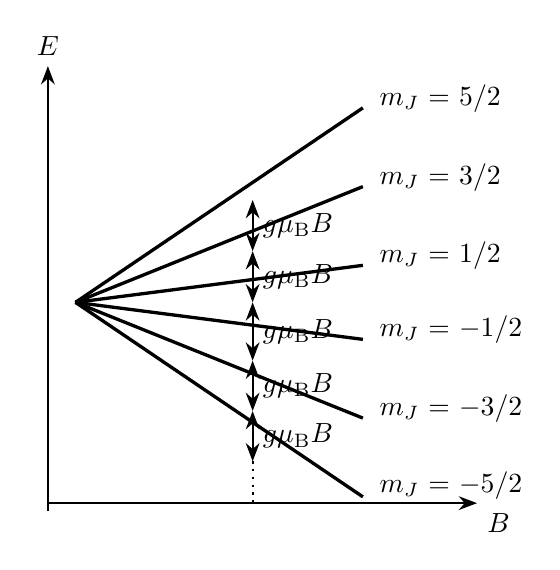
\begin{tikzpicture}[line width=0.8pt,>=Stealth]
% axes
\draw[->] (0,-0.1) -- (0,5.55) node[above] {$E$};
\draw[->] (0,0) -- (5.45,0) node[below right] {$B$};
% fan apex at B=0
\coordinate (A) at (0.35,2.55);
% six straight levels
\draw[very thick] (A) -- (4.0,5.02);
\draw[very thick] (A) -- (4.0,4.02);
\draw[very thick] (A) -- (4.0,3.02);
\draw[very thick] (A) -- (4.0,2.08);
\draw[very thick] (A) -- (4.0,1.08);
\draw[very thick] (A) -- (4.0,0.08);
% right-hand labels
\node[anchor=west] at (4.08,5.14)  {$m_J$ = $5/2$};
\node[anchor=west] at (4.08,4.14)  {$m_J$ = $3/2$};
\node[anchor=west] at (4.08,3.14)  {$m_J$ = $1/2$};
\node[anchor=west] at (4.08,2.20)  {$m_J$ = $-1/2$};
\node[anchor=west] at (4.08,1.20)  {$m_J$ = $-3/2$};
\node[anchor=west] at (4.08,0.22) {$m_J$ = $-5/2$};
% double-headed arrows at fixed B between adjacent levels
\draw[<->] (2.6,3.85) -- (2.6,3.20) node[midway,right] {$g\mu_{\mathrm{B}}B$};
\draw[<->] (2.6,3.20) -- (2.6,2.55) node[midway,right] {$g\mu_{\mathrm{B}}B$};
\draw[<->] (2.6,2.55) -- (2.6,1.81) node[midway,right] {$g\mu_{\mathrm{B}}B$};
\draw[<->] (2.6,1.81) -- (2.6,1.17) node[midway,right] {$g\mu_{\mathrm{B}}B$};
\draw[<->] (2.6,1.17) -- (2.6,0.53) node[midway,right] {$g\mu_{\mathrm{B}}B$};
% dotted vertical from lowest level down to B axis
\draw[dotted] (2.6,0.53) -- (2.6,0);
\end{tikzpicture}
\end{document}
